\section{Lighting the LED from Scilab}
\subsection{Lighting the LED}
\label{sec:light-sci}
In this section, we discuss how to carry out the experiments of the
previous section from Scilab.  We will list the same four experiments,
in the same order.  The Shield has to be attached to the \arduino\ board
before doing these experiments and the \arduino\ needs to be connected to the computer 
with a USB cable, as shown in \figref{arduino}.
The reader should go through the instructions given in
\secref{sec:sci-start} before getting started. 
\begin{enumerate}
  \item In the first experiment, we will light up the blue LED on the
        Shield.  The code for this is given in \sciref{sci:led-blue}.  It
        begins with a command of the form
        \begin{lstlisting}[style=nonumbers]
     ok = open_serial(1, PORT NUMBER, BAUD RATE)
  \end{lstlisting}
        We have used 2 for {\tt PORT NUMBER} and 115200 for {\tt BAUD RATE}.
        As a result, this command becomes
        \lstinputlisting[firstline=1,lastline=1]{\LocLEDscicode/led-blue.sce}
        This command is used to open the serial port.  When the port is
        opened successfully, it returns a value of 0, which gets stored in
        the variable {\tt ok}.
        
        Sometimes, the serial port does not open, as mentioned in the above
        command.  This is typically due to not closing the serial port
        properly in a previous experiment.  If this condition is not
        trapped, the program will wait forever, without any information
        about this difficulty.  One way to address this difficulty is to
        terminate the program if the serial port does not open.  This is
        achieved using the error message of the following form:
        \begin{lstlisting}[style=nonumbers]
     if ok ~= 0, error(Error Message in Quotes);
  \end{lstlisting}
        It checks if {\tt ok = 0}.  If not, it flashes an error message and
        terminates.  This line gets implemented in the following way in
        \sciref{sci:led-blue}.  
        \lstinputlisting[firstline=2,lastline=2]{\LocLEDscicode/led-blue.sce}
        
        We turn the LED on in the next line.  This is achieved using a
        command of the form
        \begin{lstlisting}[style=nonumbers]
    cmd_digital_out(1, PIN NUMBER, VALUE)
  \end{lstlisting}
        As we want to turn on the blue light in the Shield, as discussed in
        \secref{sec:light-ard}, we choose {\tt PIN NUMBER} as 9.  We can put
        any positive integer in the place of {\tt VALUE}.  We arrive at the
        following command:
        \lstinputlisting[firstline=3,lastline=3]{\LocLEDscicode/led-blue.sce}
        
        The last line in the code closes the serial port.  As mentioned
        above, it is extremely important to close the serial port properly.
        If not closed properly, there could be difficulties in running
        subsequent programs.
        
  \item \sciref{sci:led-blue-delay} does the same thing as what
        \ardref{ard:led-blue-delay} does.  It does two more things than what
        \sciref{sci:led-blue} does: It makes the blue LED light up for two
        seconds.  This is achieved by the command
        \lstinputlisting[firstline=4,lastline=4]{\LocLEDscicode/led-blue-delay.sce}
        The second thing this code does is to turn the blue LED off.  This
        is achieved by the command
        \lstinputlisting[firstline=5,lastline=5]{\LocLEDscicode/led-blue-delay.sce}
        It is easy to see that this code puts a 0 on pin 9.
        
  \item \sciref{sci:led-blue-red} does the same thing as what
        \ardref{ard:led-blue-red} does.  It turns blue and red LEDs on for
        five seconds.  After that, it turns off blue first.  After 3
        seconds, it turns off red also.  So, when the program ends, no LED is
        lit up.
        
  \item \sciref{sci:led-green-blink} does exactly what its counterpart
        in the Arduino IDE does.  It makes the green LED blink five times.
\end{enumerate}

\begin{exercise}
  Repeat the exercise of the previous section.
\end{exercise}

\subsection{Scilab Code}
\lstset{style=mystyle}
\label{sec:led-scilab-code}
\addtocontents{cod}{\protect\addvspace{\codclr}}

\begin{scicode}
  \ccaption{Turning on the blue LED}
  {Turning on the blue LED.  Available at
    \LocLEDscibrief{led-blue.sce}.}
  \label{sci:led-blue}
  \lstinputlisting{\LocLEDscicode/led-blue.sce}
\end{scicode}

\begin{scicode}
  \ccaption{Turning on the blue LED and turning it off after two
    seconds}{Turning on the blue LED and turning it off after two
    seconds.  Available  
    at \LocLEDscibrief{led-blue-delay.sce}.}
  \label{sci:led-blue-delay}
  \lstinputlisting{\LocLEDscicode/led-blue-delay.sce}
\end{scicode}

\begin{scicode}
  \ccaption{Turning on blue and red LEDs for 5 seconds and then turning
    them off one by one}{Turning on blue and red LEDs for 5 seconds and
    then turning them off one by one.  Available at
    \LocLEDscibrief{led-blue-red.sce}.}
  \label{sci:led-blue-red}
  \lstinputlisting{\LocLEDscicode/led-blue-red.sce}
\end{scicode}

\begin{scicode}
  \ccaption{Blinking the green LED}{Blinking the green LED.  Available
    at \LocLEDscibrief{led-green-blink.sce}.}
  \label{sci:led-green-blink}
  \lstinputlisting{\LocLEDscicode/led-green-blink.sce}
\end{scicode}


\section{Lighting the LED from Scilab Xcos}
\label{sec:light-xcos}
In this section, we will see how to light the LEDs from Scilab Xcos.
We will carry out the same four experiments as in the previous
sections.  For each, we will give the location
of the zcos file and the parameters to set.  The reader should go
through the instructions given in \secref{sec:xcos-start} before
getting started.

\begin{enumerate}
  \item First we will see how to turn on the blue LED.  When the file
        required for this experiment is invoked, one gets the GUI as in 
        \figref{fig:led-blue}.  In the caption of this figure, one can see
        where to locate the file.
        
        \begin{figure}
          \centering
          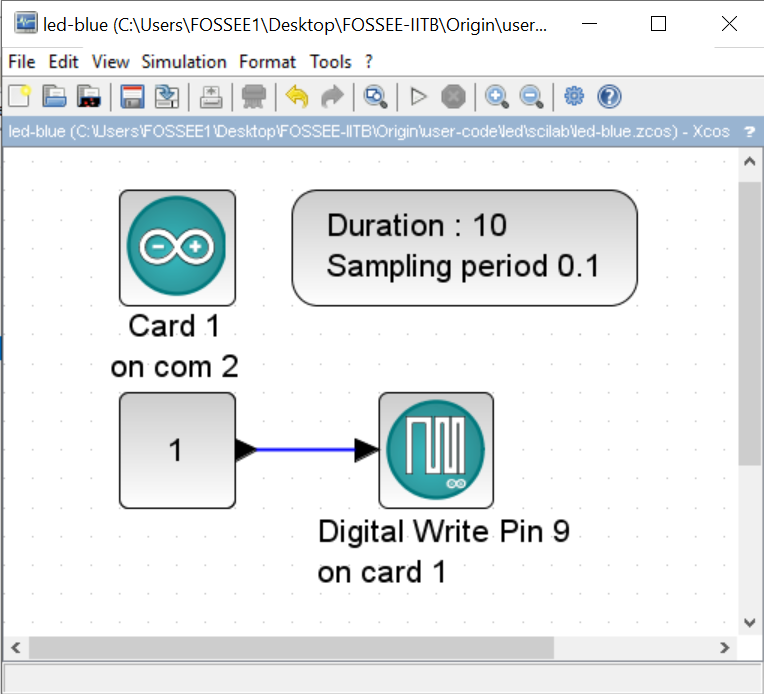
\includegraphics[width=\smfig]{\LocLEDfig/led-blue-com-2.png}
          \caption[Turning the blue LED on through Xcos]{Turning the blue
            LED on through Xcos.  This is what one sees when
            \LocLEDscibrief{led-blue.zcos} is invoked.}
          \label{fig:led-blue}
        \end{figure}
        
        We will next explain how to set the parameters for this simulation.
        To set value on any block, one needs to right click and open the
          {\tt Block Parameters} or double click.  The values for each block
        is tabulated in \tabref{tab:led-blue}.  All other parameters are to
        be left unchanged.
        \begin{table}
          \centering
          \caption{Parameters to light the blue LED in Xcos}
          \label{tab:led-blue}
          \begin{tabular}{lp{2.5cm}p{2.5cm}} \hline
            Name of the block  & Parameter name             & Value     \\ \hline
            ARDUINO\_SETUP     & Identifier of Arduino Card & 1         \\
                               & Serial com port number     & 2\portcmd \\ \hline
            TIME\_SAMPLE       & Duration of acquisition(s) & 10        \\
                               & Sampling period(s)         & 0.1       \\ \hline
            DIGITAL\_WRITE\_SB & Digital pin                & 9         \\
                               & Arduino card number        & 1         \\ \hline
          \end{tabular}
        \end{table}
        
  \item In the second experiment, we will show how to turn on the blue LED on
        for two seconds and then to turn it off.  When the file required for
        this experiment is invoked, one gets the GUI as in
        \figref{fig:led-blue-delay}.  In the caption of this figure, one can
        see where to locate the file.
        
        \begin{figure}
          \centering
          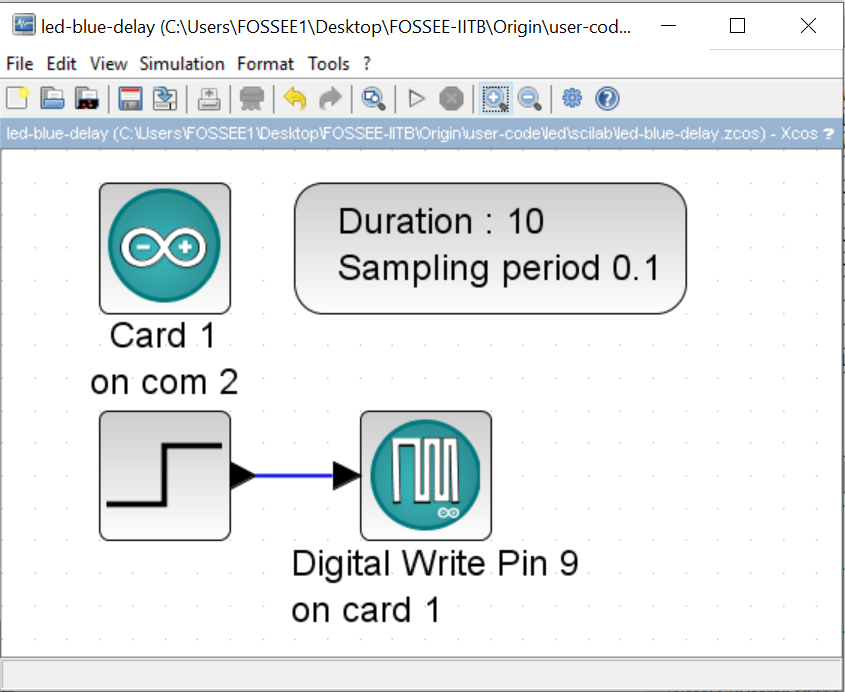
\includegraphics[width=\smfig]{\LocLEDfig/led-blue-delay-com-2.png}
          \caption[Turning the blue LED on through Xcos for two
            seconds]{Turning the blue LED on through Xcos for two
            seconds.  This is what one sees when
            \LocLEDscibrief{led-blue-delay.zcos} is invoked.}
          \label{fig:led-blue-delay}
        \end{figure}
        
        The values for each block required in this program are tabulated in
        \tabref{tab:led-blue-delay}.  All other parameters are to be left
        unchanged.
        \begin{table}
          \centering
          \caption{Parameters to light the blue LED in Xcos for two seconds}
          \label{tab:led-blue-delay}
          \begin{tabular}{lp{2.5cm}p{2.2cm}} \hline
            Name of the block  & Parameter name             & Value     \\ \hline
            ARDUINO\_SETUP     & Identifier of Arduino Card & 1         \\
                               & Serial com port number     & 2\portcmd \\ \hline
            TIME\_SAMPLE       & Duration of acquisition(s) & 10        \\
                               & Sampling period(s)         & 0.1       \\ \hline
            DIGITAL\_WRITE\_SB & Digital pin                & 9         \\
                               & Arduino card number        & 1         \\ \hline
            STEP\_FUNCTION     & Step time                  & 2         \\
                               & Initial value              & 1         \\
                               & Final value                & 0         \\ \hline
          \end{tabular}
        \end{table}
        
  \item In the third experiment, we will show how to turn the blue LED
        and the red LED on for five seconds, turn off the blue LED and three
        seconds later, turn off the red LED also.  When the file required for
        this experiment is invoked, one gets the GUI as in
        \figref{fig:led-blue-red}.  In the caption of this figure, one can
        see where to locate the file.
        
        \begin{figure}
          \centering
          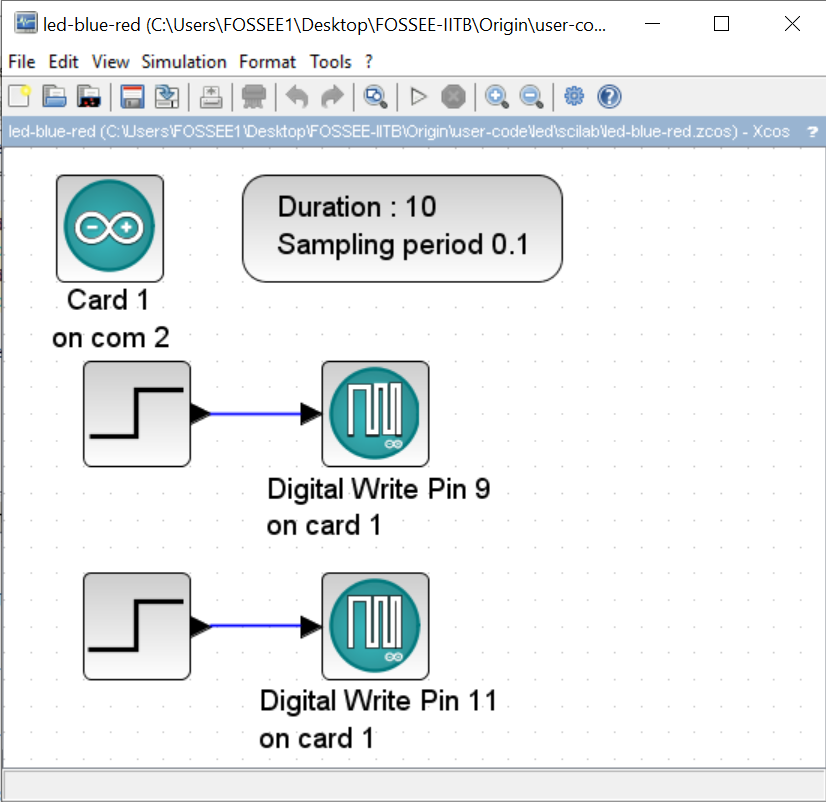
\includegraphics[width=\smfig]{\LocLEDfig/led-blue-red-com-2.png}
          \caption[Turning the blue and red LEDs on through Xcos and turning
            them off one by one]{Turning the blue and red LEDs on through
            Xcos and turning them off one by one.  This is what one sees
            when \LocLEDscibrief{led-blue-red.zcos} is invoked.}
          \label{fig:led-blue-red}
        \end{figure}
        
        The values for each block required in this program are tabulated in
        \tabref{tab:led-blue-red}.  All other parameters are to be left
        unchanged.
        \begin{table}
          \centering
          \caption{Parameters to turn the blue and red LEDs on and then turn
            them off one by one}
          \label{tab:led-blue-red}
          \begin{tabular}{lp{2.5cm}p{2cm}} \hline
            Name of the block    & Parameter name             & Value     \\ \hline
            ARDUINO\_SETUP       & Identifier of Arduino Card & 1         \\
                                 & Serial com port number     & 2\portcmd \\ \hline
            TIME\_SAMPLE         & Duration of acquisition(s) & 10        \\
                                 & Sampling period(s)         & 0.1       \\ \hline
            DIGITAL\_WRITE\_SB 1 & Digital pin                & 9         \\
                                 & Arduino card number        & 1         \\ \hline
            STEP\_FUNCTION 1     & Step time                  & 5         \\
                                 & Initial value              & 1         \\
                                 & Final value                & 0         \\ \hline
            DIGITAL\_WRITE\_SB 2 & Digital pin                & 11        \\
                                 & Arduino card number        & 1         \\ \hline
            STEP\_FUNCTION 2     & Step time                  & 8         \\
                                 & Initial value              & 1         \\
                                 & Final value                & 0         \\ \hline
          \end{tabular}
        \end{table}
        
  \item We will conclude this section with an experiment to blink the
        green LED on and off.  When the file required for
        this experiment is invoked, one gets the GUI as in
        \figref{fig:led-green-blink}.  In the caption of this figure, one can
        see where to locate the file.
        
        \begin{figure}
          \centering
          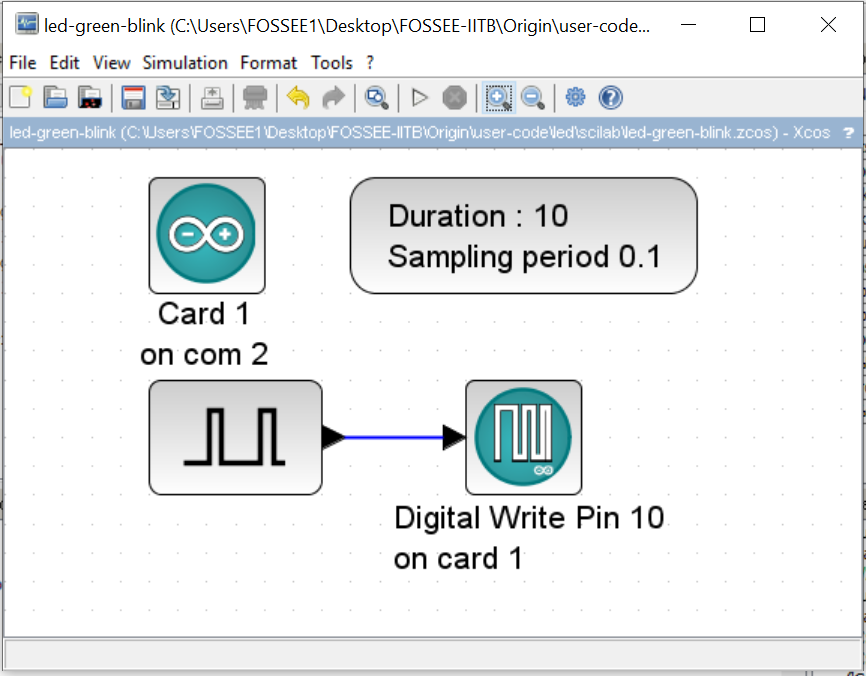
\includegraphics[width=\smfig]{\LocLEDfig/led-green-blink-com-2.png}
          \caption[Blinking the green LED every second through
            Xcos]{Blinking the green LED every second through Xcos.
            This is what one sees when
            \LocLEDscibrief{led-green-blink.zcos} is invoked.}
          \label{fig:led-green-blink}
        \end{figure}
        
        The values for each block required in this program are tabulated in
        \tabref{tab:led-green-blink}.  All other parameters are to be left
        unchanged.
        \begin{table}
          \centering
          \caption{Parameters to make the green LED blink every second}
          \label{tab:led-green-blink}
          \begin{tabular}{lp{2.5cm}p{2.5cm}} \hline
            Name of the block  & Parameter name             & Value     \\ \hline
            ARDUINO\_SETUP     & Identifier of Arduino Card & 1         \\
                               & Serial com port number     & 2\portcmd \\ \hline
            TIME\_SAMPLE       & Duration of acquisition(s) & 10        \\
                               & Sampling period(s)         & 0.1       \\ \hline
            DIGITAL\_WRITE\_SB & Digital pin                & 10        \\
                               & Arduino card number        & 1         \\ \hline
            PULSE\_SC          & Pulse width(\% of period)  & 50        \\
                               & Period(secs)               & 2         \\ 
                               & Phase delay(secs)          & 0.1       \\
                               & Amplitude                  & 1         \\ \hline
          \end{tabular}
        \end{table}
\end{enumerate}

% \section{Control through Xcos}
% This experiment implements digital write functionality of Arduino board.
% % \begin{figure}
% % \centering
% % 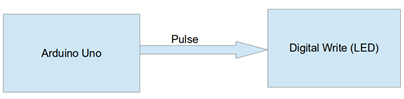
\includegraphics[width=\smfig]{\LocLEDfig/xcos-wri.png}
% % \caption{Digital write functionality}
% % \label{fig:xcoswri}
% % \end{figure}

% \begin{figure}
% \centering
% 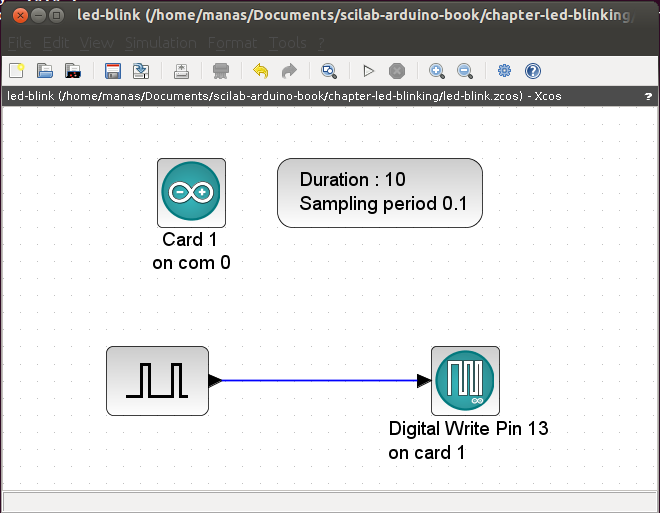
\includegraphics[width=\smfig]{\LocLEDfig/xcos-led.png}
% \caption{Xcos diagram for LED interfacing}
% \label{fig:xcosblk}
% \end{figure}

% \begin{figure}
% \centering
% 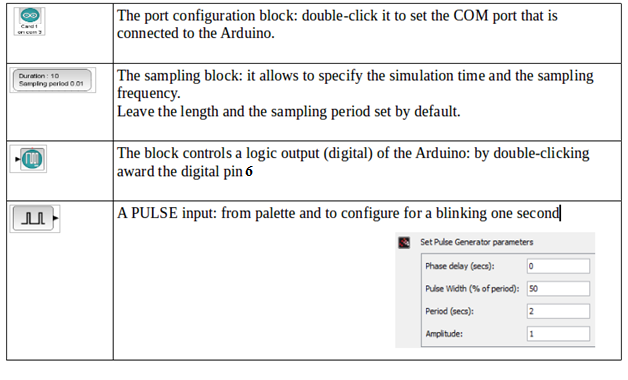
\includegraphics[width=\smfig]{\LocLEDfig/xcos-desc.png}
% \caption{Xcos blocks}
% \label{fig:xcosdesc}
% \end{figure}

% \section{Experiment: Blink LED for limited number of iterations}
% This experiment is about continuous switching on and switching off the LED a fixed number of times. Here we use  for loop to carry out limited number of iterations of the code.  The structure of for loop is:

% \begin{lstlisting}      
% for variable = start_point:end_point
%    instructions
% end
% \end{lstlisting}   

% Here variable is incremented by 1 in every iteration, till the condition variable=end\_point is met. Thus before each iteration, the above condition is verified. Figure shows the flow-chart of the operation.
% \begin{figure}
% \centering
% \includegraphics[width=\smfig]{\LocLEDfig/LEDflowchart.png}
% \caption{Flow chart}
% \label{fig:ledfc}
% \end{figure}



\begin{exercise}
  Carry out the following exercise:
  \begin{enumerate}
    \item Change the blink pattern for an array of LEDs.
    \item Change the delays.
  \end{enumerate}
\end{exercise}

